% !TEX root =  ../Dissertation.tex

\chapter{Software Design and Implementation}

This section discusses the existing tools in robotics and HRI research, namely Robot Operating System (ROS), ROS4HRI, and OfficeBots, and elaborates on the design principles and implementation specifics of the culturally aware robotic framework, which builds upon the foundational ROS and its extension ROS4HRI for Human-Robot Interaction (HRI) research.

\section{Robot Operating System (ROS)}

The Robot Operating System (ROS) is a flexible, open-source framework that has become a cornerstone in robotics software development. This middleware provides fundamental services for hardware abstraction, low-level device control, implementation of commonly used functionality, message-passing between processes, and package management. Its utility in facilitating message passing and service calls through topics and services has catalysed the advancement and democratization of robotics research and development.

\section{ROS4HRI}

With the advent of the ROS4HRI extension in October 2022, the application of ROS has further expanded into the domain of Human-Robot Interaction. This enhancement to ROS standardizes topics and conventions specifically tailored for HRI, encompassing critical functionalities such as face detection, body tracking, and other key interactive features. ROS4HRI serves as an invaluable bridge between the traditionally robotic-centric focus of ROS and the nuanced requirements of social robotics.

\section{OfficeBots}

OfficeBots emerges as an innovative tool to facilitate HRI research, manifesting as a 3D simulation environment modelled after an office. Supporting both research and educational endeavours, OfficeBots enables users to navigate a virtual space featuring interactable objects and robotic agents. Through this tool, researchers can experiment with robot augmentation, behavioural modification, and interaction in a controlled, reproducible setting that closely mirrors real world scenarios.

\section{Architecture}

The system architecture is structured as a multi-tiered framework, where each layer fulfills distinct functions and interacts through well defined interfaces:

\begin{itemize}
    \item \textbf{ROS Core:} Serving as the fundamental communication medium, ROS facilitates message passing between nodes and manages services and actions within the robotic environment.
    \item \textbf{ROS4HRI:} Extending core ROS functionalities, ROS4HRI introduces dedicated nodes and topics for human-robot interaction capabilities, enriching the system with features like motion tracking and body movement detection.
    \item \textbf{Culturally Aware Extensions:} These custom nodes and services, developed atop ROS and ROS4HRI, imbue robotic behaviors with cultural awareness. They enable adaptations based on participant input regarding nationality and cultural preferences. Notably, the implementation integrates the factory pattern, anticipating future extensions to explore additional cultural values such as race and gender.
\end{itemize}

\subsection{Factory Pattern}

This project strategically employs factory pattern in achieving flexibility and scalability within the framework. It enables dynamic object creation without the need for specifying their exact classes. Applied in both the robot and database components, this pattern allows for seamless customisation and adaptation to diverse cultural contexts.

\begin{figure}
    \begin{center}
        \noindent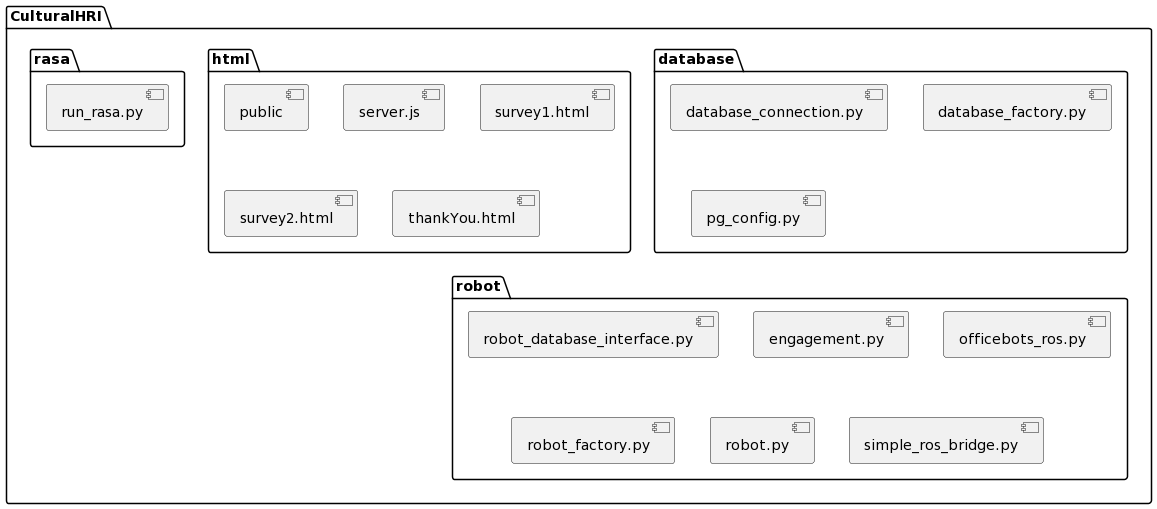
\includegraphics[width=\linewidth]{Chapter6/package.png}  
        \caption{System Architecture of the Culturally Aware Robotic Framework.}
        \label{fig:figure1}
    \end{center}
\end{figure}

\begin{figure}
   \noindent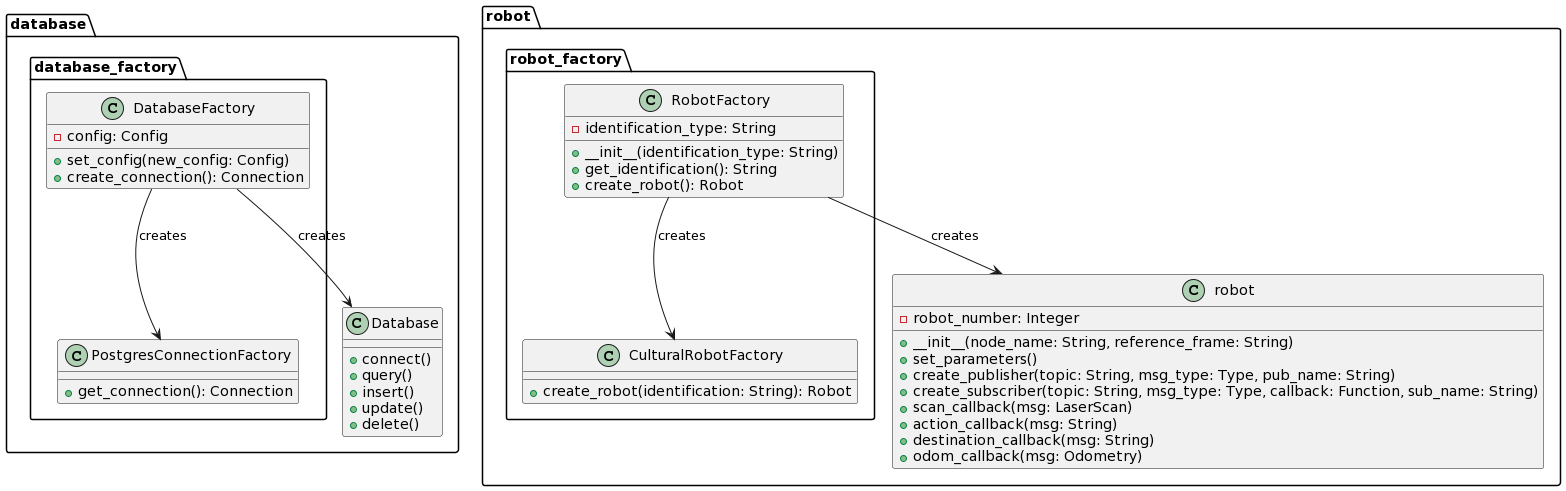
\includegraphics[width=\linewidth]{Chapter6/factory.png}  
   \caption{Factory Pattern Implementation in the Framework for easy extension and customisation.}
  \label{fig:figure2}
\end{figure}

\subsubsection{Robot Factory}

The robot factory dynamically creates instances of robot objects based on specific criteria such as the cultural context or nationality of users. This flexibility empowers the framework to instantiate different types of robots with varied behaviours tailored to specific cultural parameters.

\subsubsection{Database Factory}

Similarly, the database factory is responsible for generating database connections tailored to specific database types (e.g., PostgreSQL). By abstracting the process of connection creation, it allows for seamless switching between different database systems or configurations, enhancing adaptability for future experiments.

By employing the factory pattern in this project, the framework enables easy manipulation, extendibility, and customisation of the creation of database connections and robots without modifying existing code. Such a pattern enables a more flexible and adaptable implementation for future changes and experiments involving different cultural values or behaviours.

\section{Programming Languages and Technologies}

To fulfil its functional and experimental objectives, the project harnesses a diverse array of programming languages and software stacks:

\begin{itemize}
    \item \textbf{Python:} Primarily utilized for ROS node development, Python defines robot behaviors through subscribers and publishers. Additionally, it integrates with RASA Conversational AI for natural language interactions and Flask web framework for HTTP request handling and survey data processing.
    \item \textbf{JavaScript:} Drives frontend development for surveys, facilitating a dynamic user interface, and is utilized on the backend for data collection and relay to the Flask server and robotic framework.
    \item \textbf{SQL:} Employed to structure the Postgres database schema storing survey data essential for configuring robot behaviors aligned with cultural contexts.
    \item \textbf{C\#:} Powers the OfficeBots environment within the GoDot game engine, enabling high-fidelity simulation for HRI studies and implementing multilingual support for cultural interaction within the simulation.
\end{itemize}

\section{Integration and Communication}

The project's integration strategy ensures smooth communication between the survey interface, data storage, and the robotic environment:

\begin{itemize}
    \item \textbf{Data Flow:} Survey responses collected via the JavaScript frontend are stored in the Postgres database. SQL queries retrieve this data, which is then passed through the Flask interface to ROS, facilitating the translation of survey responses into robotic actions.
    \item \textbf{ROS Bridge:} Serving as the conduit between web-based components (Flask server) and ROS/ROS4HRI systems, the ROS Bridge facilitates seamless communication.
    \item \textbf{Simulation Interaction:} C\# scripts within the GoDot game engine translate transmitted data into live changes, updating robot behavior in the OfficeBots environment to reflect cultural adaptations.
\end{itemize}

\begin{figure}
    \begin{center}
        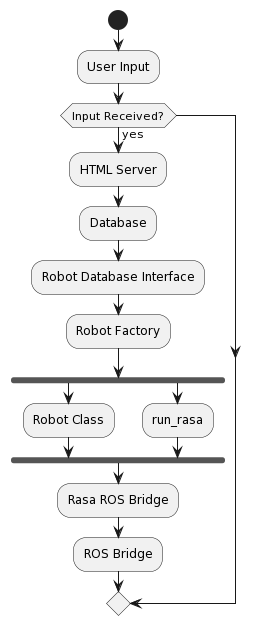
\includegraphics[scale=0.5]{Chapter6/flow.png}  
        \caption{Data Flow and Communication between the Survey Interface, Database, and Robot Class.}
        \label{fig:figure3}
    \end{center}
\end{figure}

\section{Development Environment}

Modular development is adopted to allow independent testing and deployment:

\begin{itemize}
    \item \textbf{Version Control:} Git effectively manages code changes and collaboration.
    \item \textbf{Development Tools:} Various IDEs and editors are employed, tailored for respective languages such as PyCharm for Python, and Visual Studio Code for JavaScript and C\#.
    \item \textbf{Testing Frameworks:} Utilization of unit-testing and integration testing frameworks ensures the reliability and correctness of individual components and their integration. The employment of the factory pattern anticipates future extensions, providing a flexible and scalable framework for cultural adaptation in HRI experiments.
\end{itemize}

\section{Testing}

Utilization of unit-testing and integration testing frameworks ensures the reliability and correctness of individual components and their integration. The employment of the factory pattern anticipates future extensions, providing a flexible and scalable framework for cultural adaptation in HRI experiments.

In the testing phase, unit tests were conducted for individual functions and classes within these scripts. Integration tests were also performed to assess the interaction between these components. Notably, the testing process revealed the reliability of the framework, particularly in scenarios where the \texttt{RobotFactory} class interacts with the \texttt{DatabaseFactory} class.

\subsection{Unit Testing}

The database module comprises scripts responsible for managing database connections and configurations. Similarly, within the robot module, scripts oversee robotic engagement, interface with databases, and control robot behavior. Additionally, the rasa module contains scripts dedicated to running the Rasa conversational AI platform.

The factory pattern plays a crucial role within the robot and database modules. For instance, the \texttt{RobotFactory} class in the \texttt{robot\_factory.py} script facilitates the creation of various types of robots, while the \texttt{DatabaseFactory} class in the \texttt{database\_factory.py} script enables the creation of different database connections.

During testing, it was noted that the database module effectively manages database connections and configurations, while the robot module adeptly handles robotic engagement, database interfacing, and robot behaviour control. Additionally, the rasa module efficiently executes the Rasa conversational AI platform.

The implementation of the factory pattern within the robot and database modules proved to be instrumental. For example, the \texttt{RobotFactory} class in the \texttt{robot\_factory.py} script seamlessly generated various types of robots, while the \texttt{DatabaseFactory} class in the \texttt{database\_factory.py} script efficiently created different database connections.

The versatility of the factory pattern was demonstrated by simulating scenarios where non-existent classes such as \texttt{GenderRobot} and \texttt{RaceRobot} were requested for instantiation. Despite these classes not being present in the current implementation, the factory pattern demonstrated its flexibility and adaptability by handling such requests without errors or disruptions.

This exercise showcased the potential benefits of the factory pattern for future extension experiments. By allowing for the dynamic creation of objects without specifying their exact class, the factory pattern is well-suited for accommodating new types of robots or database connections as the framework evolves. This capability becomes particularly valuable in the context of cultural adaptation in Human-Robot Interaction (HRI) experiments.

In future experiments exploring gender-specific or race-specific robot behaviors, the factory pattern can facilitate the seamless integration of new, non-implemented classes such as \texttt{GenderRobot} and \texttt{RaceRobot}. This allows researchers to easily extend the framework to incorporate culturally sensitive interactions tailored to specific gender or race identities.

\subsection{Integration Testing}

Integration testing represents a pivotal stage of software assessment wherein individual units are amalgamated and examined collectively to uncover any operational anomalies stemming from their interaction.

In the context of this Human-Robot Interaction (HRI) framework project, integration testing assumes significance in assessing the seamless collaboration among various components. This evaluation encompasses scrutinising how the robot's behaviour adapts in response to different cultural parameters or how it interfaces with the database.

Systematic testing of such interactions ensures the cohesive operation of the framework's components, thereby ensuring a reliable and seamless user experience. Moreover, integration testing aids in identifying and rectifying any potential inconsistencies or issues in the integration process before deployment.

To conduct integration testing effectively, various test scenarios were devised to replicate real-world interactions between distinct modules of the framework. For instance, scenarios were evaluated where the robot retrieved cultural parameters from the database to inform its behaviour, or where the robot's state was stored and later retrieved for analysis.